\documentclass[a4paper, 11pt]{article}
\usepackage[left=2cm,right=2cm,top=2cm,bottom=2cm]{geometry}
\setlength{\parindent}{1cm}
\usepackage{graphicx}
\usepackage{kvsetkeys}
\begin{document}

\title{MM2090 Assignment 4}
\author{Amar Muhammed ME20B022}
\date{June 2021}
\maketitle

\section{The Equation}

\textbf{Van der Waals Equation:}  

\begin{equation}
 {\LARGE{\textbf{$(P + \frac{an^2}{V^2})(V-nb) = nRT$}}}
 \label{eq:1}
\end{equation}


\subsection{Analysis}
Following contains a brief explanation of the variables and the importance of the equation :
\begin{itemize}

    {\normalsize {The equation \ref{eq:1}  has terms \textbf{P} ,\textbf{V} , \textbf{n},\textbf{R} ,\textbf{T} ,\textbf{a} and \textbf{b}.}}\\

{\normalsize { Here,}}\\
{\normalsize {\textbf{P} represents the pressure of the system  }}\\
{\normalsize {\textbf{V} \  represents the volume of the system}}\\
{\normalsize {\textbf{n} \  represents the number of moles of gas present in the system}}\\
{\normalsize {\textbf{R} \  represents the universal gas constant}}\\
{\normalsize{\textbf{T} \ represents the temperature of the system}}\\
{\normalsize{\textbf{a} \ represents the Van der Waals constant that provides the correction for intermolecular forces.}}\\
{\normalsize{\textbf{b} \ represents the Van der Waals constant that adjusts for the volume occupied by gas molecules in the system}}
\end{itemize}


The Van der Waals equation is an equation of state that generalizes the ideal gas law based on plausible reasons that real gases do not act ideally.The ideal gas law treats gas molecules as point particles that interact with their containers but not each other, meaning they neither take up space nor change kinetic energy during collisions.
It is available via its traditional derivation (a mechanical equation of state), or via a derivation based in statistical thermodynamics, the latter of which provides the partition function of the system and allows thermodynamic functions to be specified. It successfully approximates the behavior of real fluids above their critical temperatures and is qualitatively reasonable for their liquid and low-pressure gaseous states at low temperatures. However, near the phase transitions between gas and liquid, in the range of p, V, and T where the liquid phase and the gas phase are in equilibrium, the Van der Waals equation fails to accurately model observed experimental behaviour, in particular that p is a constant function of V at given temperatures. As such, the Van der Waals model is not useful only for calculations intended to predict real behavior in regions near the critical point. Corrections to address these predictive deficiencies have since been made, such as the equal area rule or the principle of corresponding states.

\begin{figure}[h]
	{\begin{center}
		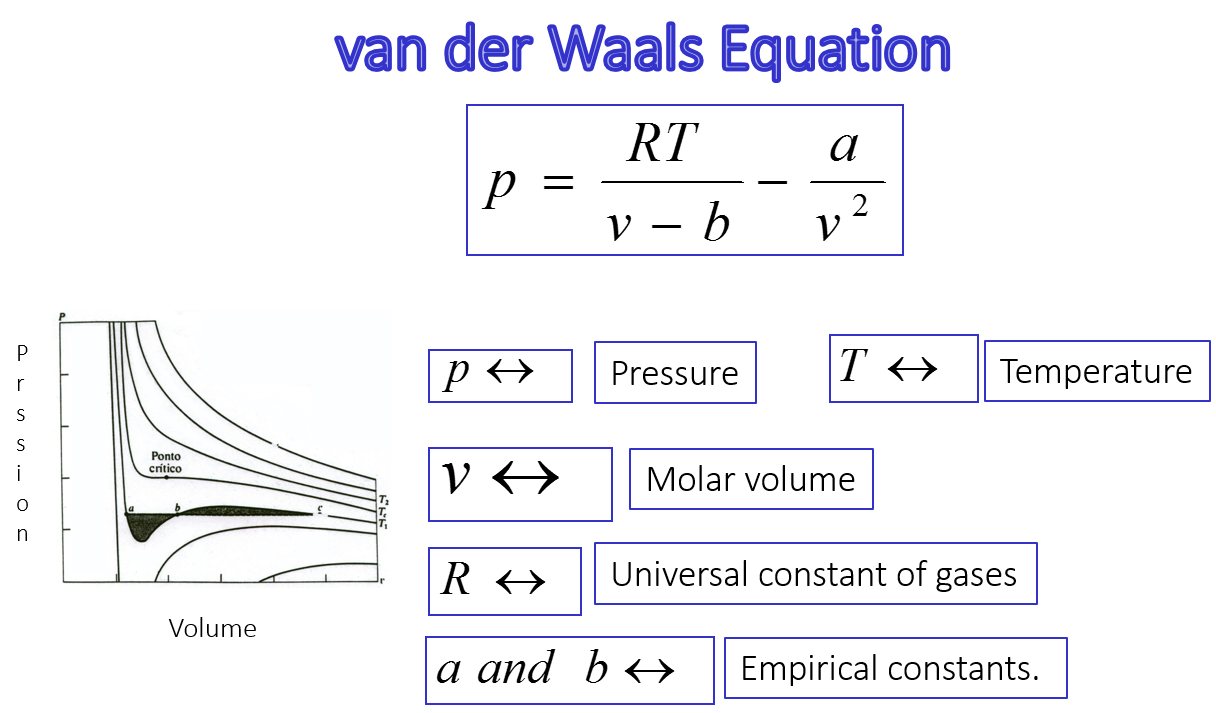
\includegraphics[scale=0.3]{me20b022.png}
	\end{center}}
	\caption{The Van der Waals equation \cite{picture}}
	\label{f1:image}
\end{figure}
\subsection{Validity}
The Van der Waals equation is mathematically simple, but it nevertheless predicts the experimentally observed transition between vapor and liquid, and predicts critical behaviour.[12]:289 It also adequately predicts and explains the Joule–Thomson effect (temperature change during adiabatic expansion), which is not possible in ideal gas.

Above the critical temperature, TC, the Van der Waals equation is an improvement over the ideal gas law, and for lower temperatures, i.e., T < TC, the equation is also qualitatively reasonable for the liquid and low-pressure gaseous states; however, with respect to the first-order phase transition, i.e., the range of (p, V, T) where a liquid phase and a gas phase would be in equilibrium, the equation appears to fail to predict observed experimental behaviour, in the sense that p is typically observed to be constant as a function of V for a given temperature in the two-phase region. This apparent discrepancy is resolved in the context of vapour–liquid equilibrium: at a particular temperature, there exist two points on the Van der Waals isotherm that have the same chemical potential, and thus a system in thermodynamic equilibrium will appear to traverse a straight line on the p–V diagram as the ratio of vapour to liquid changes. However, in such a system, there are really only two points present (the liquid and the vapour) rather than a series of states connected by a line, so connecting the locus of points is incorrect: it is not an equation of multiple states, but an equation of (a single) state. It is indeed possible to compress a gas beyond the point at which it would typically condense, given the right conditions, and it is also possible to expand a liquid beyond the point at which it would usually boil. Such states are called "metastable" states. Such behaviour is qualitatively (though perhaps not quantitatively) predicted by the Van der Waals equation of state.
\cite{website}



\bibliography{bibliography.bib}
\bibliographystyle{plain}

\end{document}
